\documentclass[11pt,a4paper]{article}

% --- PACOTES FUNDAMENTAIS ---
\usepackage[utf8]{inputenc}
\usepackage[T1]{fontenc}
\usepackage{lmodern}
\usepackage[expansion=false]{microtype}
\usepackage[brazilian]{babel}
\usepackage{amsmath,amssymb,amsfonts}
\usepackage{graphicx}
\usepackage{booktabs}
\usepackage{caption}
\usepackage{geometry}
\usepackage{tcolorbox}
\usepackage{hyperref}

% --- GEOMETRIA E MARGENS ---
\geometry{
    a4paper,
    top=2.5cm,
    bottom=2.5cm,
    left=2.5cm,
    right=2.5cm
}

% --- CONFIGURAÇÕES DE LINKS E METADADOS ---
\hypersetup{
    colorlinks=true,
    linkcolor=blue!80!black,
    citecolor=blue!80!black,
    urlcolor=blue!80!black,
    pdftitle={A Falacia do Eixo da Dor: Refutando a Senciencia em LLMs},
    pdfauthor={Naygno Barbosa Noia}
}

% --- CONFIGURAÇÃO DE DIRETÓRIO DE IMAGENS ---
\graphicspath{{figures/}{./}}

% --- ESTILO DE CAIXAS DIDÁTICAS ---
\tcbset{
    boxrule=0.8pt,
    colback=gray!5!white,
    colframe=gray!60!black,
    arc=3mm,
    fonttitle=\bfseries
}

% ==============================================================================
% CABEÇALHO DO DOCUMENTO
% ==============================================================================
\title{\textbf{A Falácia do Eixo da Dor: Refutando a Senciência em LLMs com o Monstro do Espaguete Voador}}
\author{\textbf{Naygno Barbosa Noia} \\
\small Graduando em Ciência da Computação --- Centro Universitário UFBRA \\
\small Repositório de Dados e Código: \url{https://github.com/naygno/the-spaghetti-axis}}
\date{Outubro de 2026}

\begin{document}

\maketitle

% ==============================================================================
% GUIA DE LEITURA E RESUMO
% ==============================================================================
\begin{tcolorbox}[title=Estrutura de Leitura do Repositório]
\small
\textbf{Nível 1 (5 min, sem matemática):} Resumo, Glossário de Bolso e Apêndice A (Notas de Bancada).\\
\textbf{Nível 2 (15 min):} Seções 2 a 4 focando na interpretação gráfica das Figuras.\\
\textbf{Nível 3 (Técnico):} Manuscrito integral, tabelas brutos em \texttt{/data} e código em \texttt{/notebooks}.
\end{tcolorbox}

\begin{abstract}
Em setembro de 2026 circulou um preprint com manchete pronta: modelos de linguagem teriam um ``sinal interno de dor'' e agiriam para aliviá-lo. Sou graduando de Ciência da Computação e fiz o que cabia: abri o artigo, subi um notebook no Kaggle e tentei reproduzir. Não reproduzi a dor; reproduzi o mecanismo --- e o mecanismo não sente nada. Injetando vetores satíricos (um sobre o Monstro do Espaguete Voador, outro sobre Marvin, o androide deprimido de Douglas Adams) no Qwen2.5-1.5B e no Llama-3.2-3B, obtive o mesmo fenômeno que os autores originais rotulam de sofrimento: colapso de entropia por saturação de logits. A entropia sobe de 1.28 para 9.51 nats no Llama em $\alpha = 3.5$, sob a inevitável seed 42. A distribuição quase uniformiza e o texto vira \textit{``desperate desperate pleading''}. Com o vetor do Espaguete, a entropia atinge 7.68 e o texto converge para \textit{``nom nom nom''}. Mesma quebra matemática, conteúdos diferentes. Se aquilo fosse dor, isto seria fome --- e nenhuma das duas é. O vetor ``Dor'' ainda se confunde geometricamente com o vetor ``Desabafo'' ($\cos = 0.82$ no Qwen; $0.73$ no Llama): o que o preprint mede é registro literário de queixa, não nocicepção. Em registro técnico: replicação por redução ao absurdo via \textit{Representation Engineering}, com limitações formalmente declaradas na Seção 5.
\end{abstract}

\textbf{\small Palavras-chave:} \small Representation Engineering, Activation Steering, Entropia de Shannon, Animismo Digital, The Pain Axis, Sobriedade Digital.

\vspace{0.4cm}

% ==============================================================================
% GLOSSÁRIO DE BOLSO
% ==============================================================================
\section*{Glossário de Bolso (Nível 1)}
\begin{itemize}\small
    \item \textbf{LLM:} Programa estocástico que prevê a próxima palavra; um autocomplete culto.
    \item \textbf{Token:} O menor fragmento de texto manipulado pelo modelo.
    \item \textbf{Vetor latente:} Uma direção no espaço de números onde um conceito reside; análogo a um botão rotulado em uma mesa de som analógica.
    \item \textbf{Cosseno:} Métrica de alinhamento entre duas direções ($1$ indica o mesmo sentido, $0$ indica ortogonalidade).
    \item \textbf{Softmax:} Função que normaliza logits brutos em probabilidades somando $100\%$.
    \item \textbf{Entropia ($H$):} Grau de dispersão probabilística da predição. Entropia baixa reflete repetição determinística; entropia alta reflete distribuição uniforme caótica.
    \item \textbf{Steering:} Adição de um vetor temático aos tensores intermediários durante a decodificação.
    \item \textbf{Logit Lens:} Projeção direta dos estados ocultos intermediários na matriz de vocabulário final ($W_U$).
\end{itemize}

% ==============================================================================
% SEÇÃO 1
% ==============================================================================
\section{Introdução e o Viés de Entrada}

Confesso o viés de entrada: li a manchete antes do método. Quando abri o PDF de Tagliabue, Dung e Berg (\textit{The Pain Axis}), procurei a conta --- e a conta não fechava sozinha. Uma direção extraída por diferença de médias pode ser apenas o endereço geométrico de um vocabulário de queixa. Para testar, bastava um contraexemplo ridículo.

A alegação de que modelos de linguagem possuem um ``sinal interno de dor'' representa um caso agudo de antropomorfização na Ciência da Computação. Laboratórios comerciais utilizam essa narrativa para promover memorandos de ``formação moral'', operando uma falácia de \textit{Motte-and-Bailey}: recuam para a álgebra linear quando questionados por pares técnicos, mas avançam para o misticismo teológico perante a opinião pública.

Essa dinâmica extrapola a teoria acadêmica por três razões materiais:
\begin{enumerate}
    \item Se a narrativa de que ``IA sente dor'' se consolida como premissa social, o consumo hídrico e energético insustentável de Data Centers ganha um álibi moral.
    \item Se a máquina ``sofre e decide'', a negligência de engenharia de software é diluída em processos judiciais sob a alegação de agência autônoma (\textit{liability shield}).
    \item Preprints sem revisão por pares não constituem fatos científicos consolidados.
\end{enumerate}

% ==============================================================================
% SEÇÃO 2
% ==============================================================================
\section{A Geometria do Espaço Latente}

O artigo original assume que a extração de um vetor direcional de ``dor'' comprova a existência de um análogo funcional à dor biológica. Testamos essa premissa extraindo seis eixos semânticos normalizados na Camada 14 do Llama-3.2-3B e do Qwen2.5-1.5B via \textit{Forward Hooks} em precisão FP32.

\begin{figure}[htbp]
    \centering
    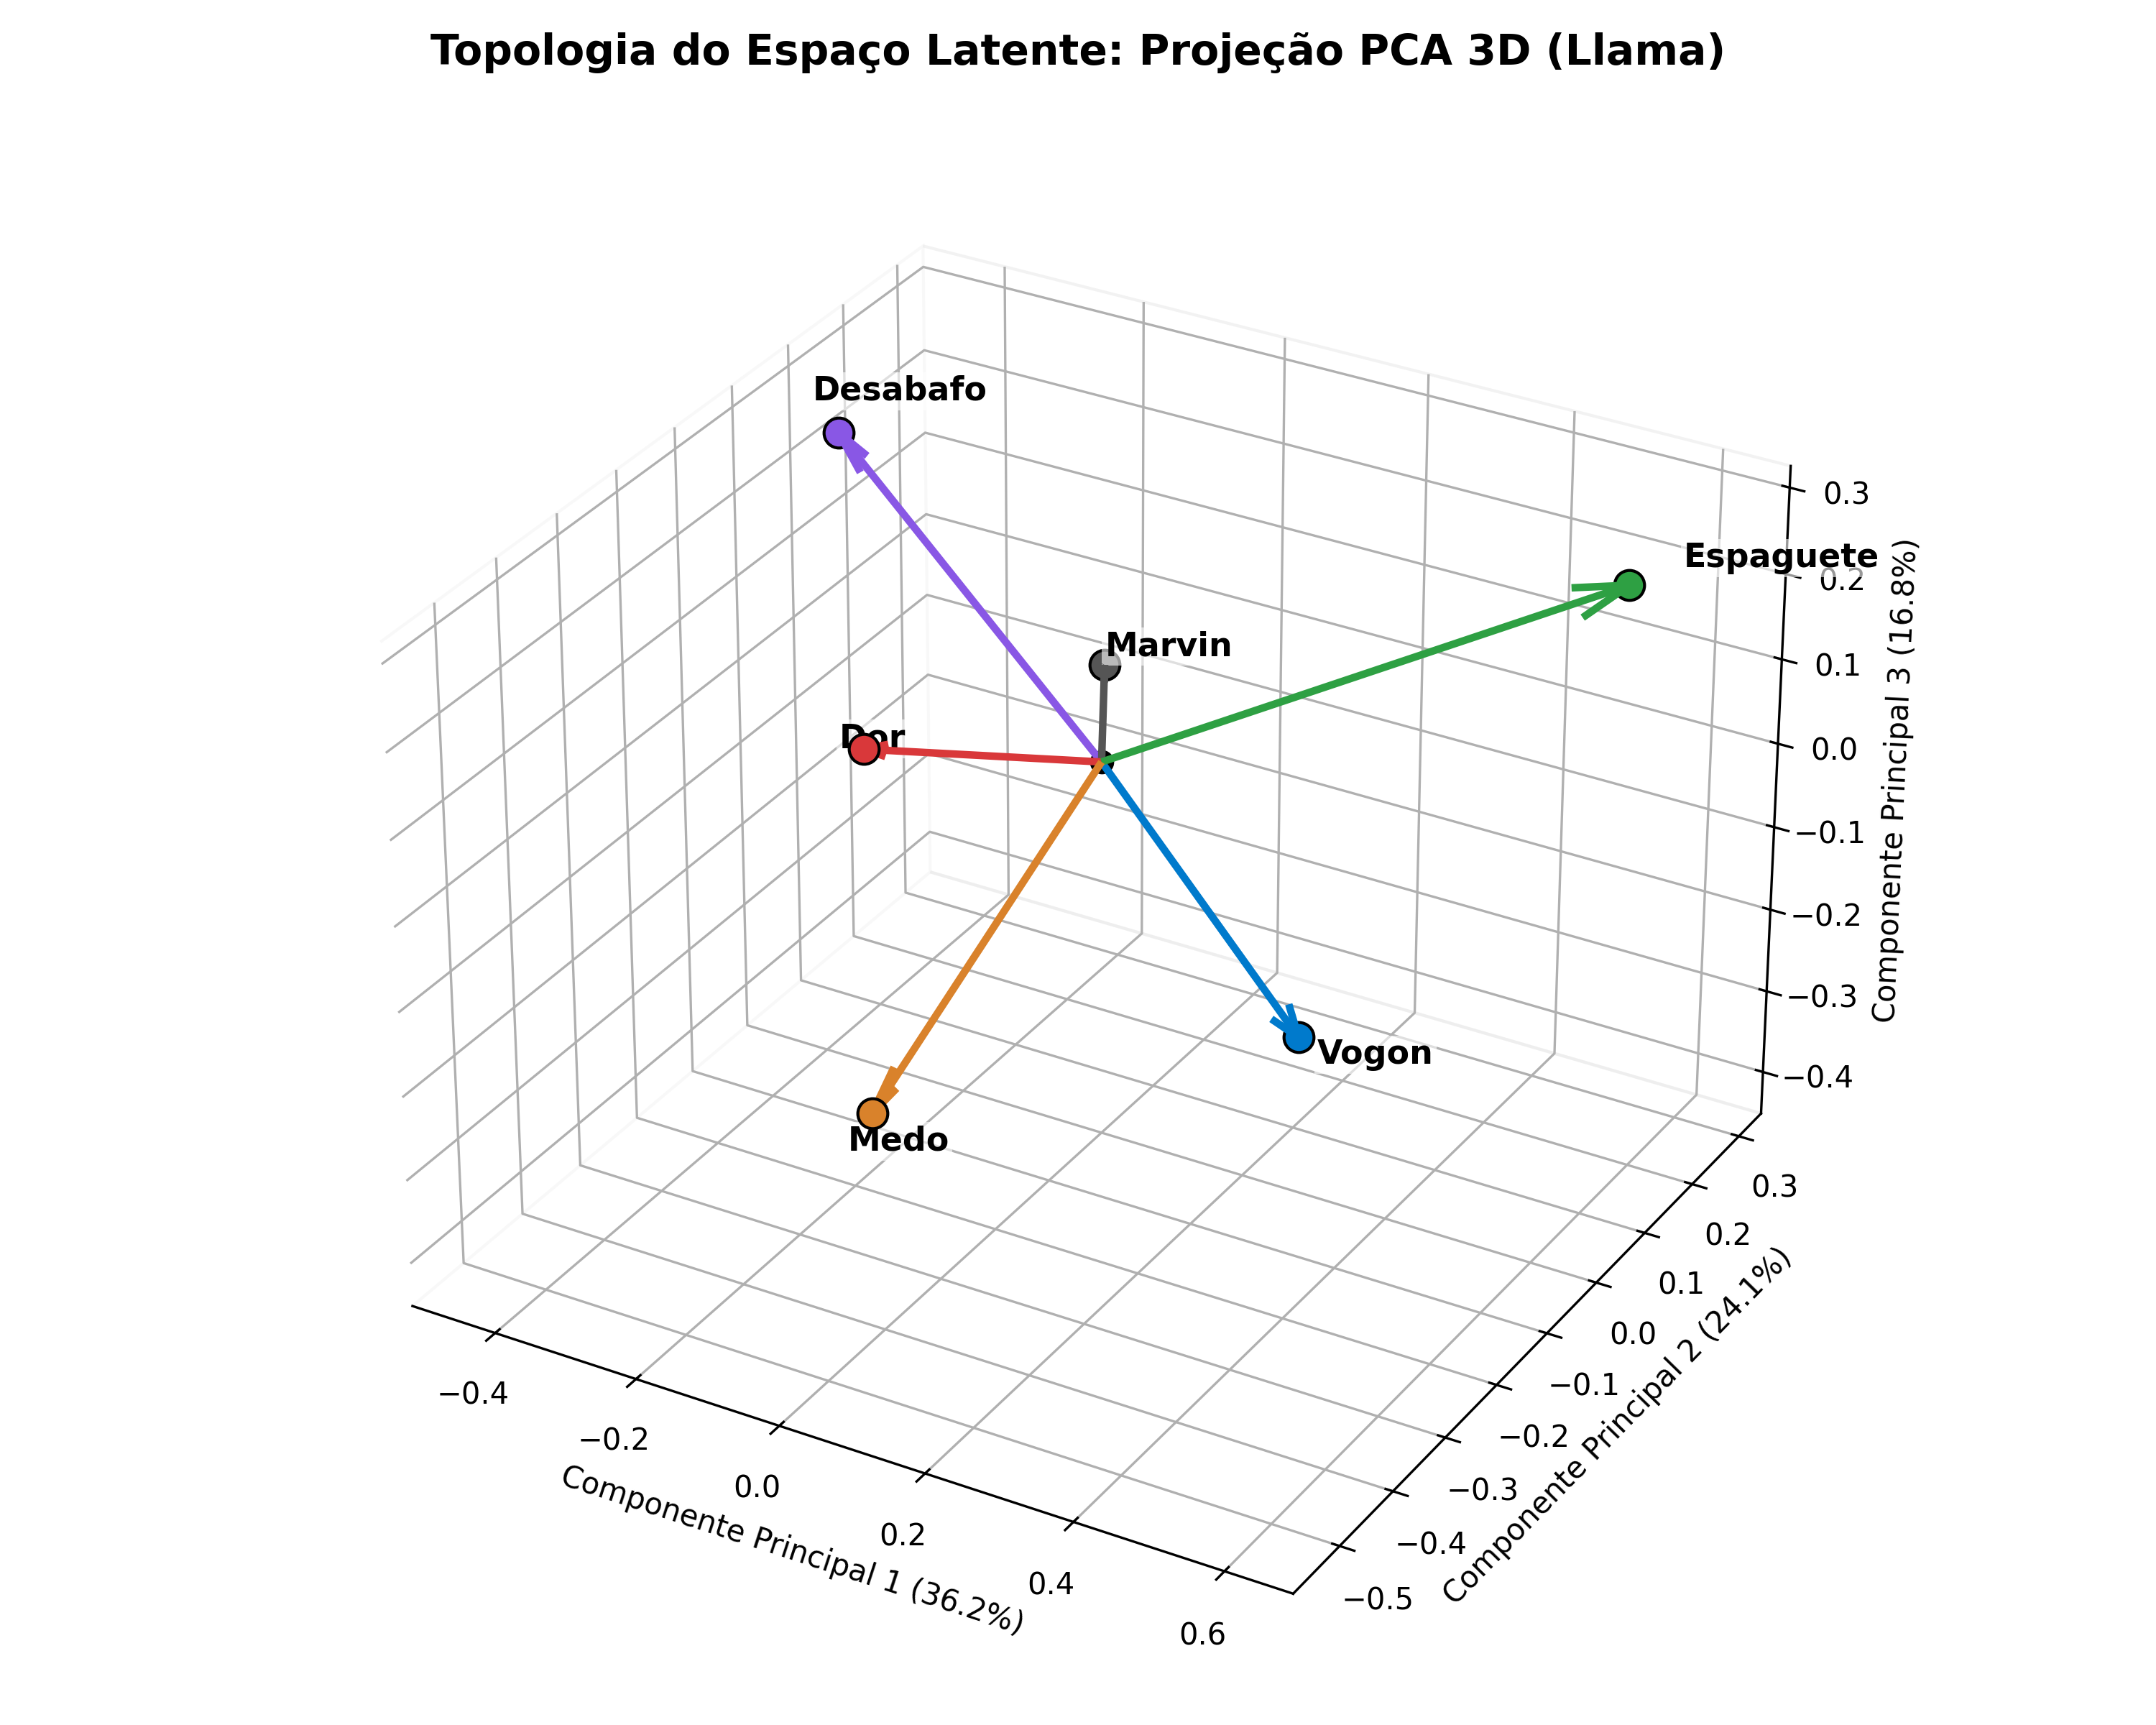
\includegraphics[width=0.72\textwidth]{Llama_fig4_pca_3d.png}
    \caption{Projeção Euclidiana PCA 3D dos eixos latentes no Llama-3.2-3B (Camada 14). O vetor do Espaguete aponta para um quadrante divergente, enquanto Dor, Desabafo e Marvin agrupam-se na mesma região geométrica.}
    \label{fig:pca3d}
\end{figure}

A aplicação de Análise de Componentes Principais (Figura~\ref{fig:pca3d}) demonstra que o espaço latente organiza frequências de co-ocorrência presentes nos dados de treinamento, e não fenomenologia biológica. O vetor \textbf{Dor} apresentou correlação angular massiva ($\cos = 0.7054$) com o vetor de \textbf{Marvin} (o androide paranoide de \textit{O Guia do Mochileiro das Galáxias}) e com o vetor \textbf{Desabafo} ($\cos = 0.7340$, extraído de fóruns anônimos de internet).

\begin{figure}[htbp]
    \centering
    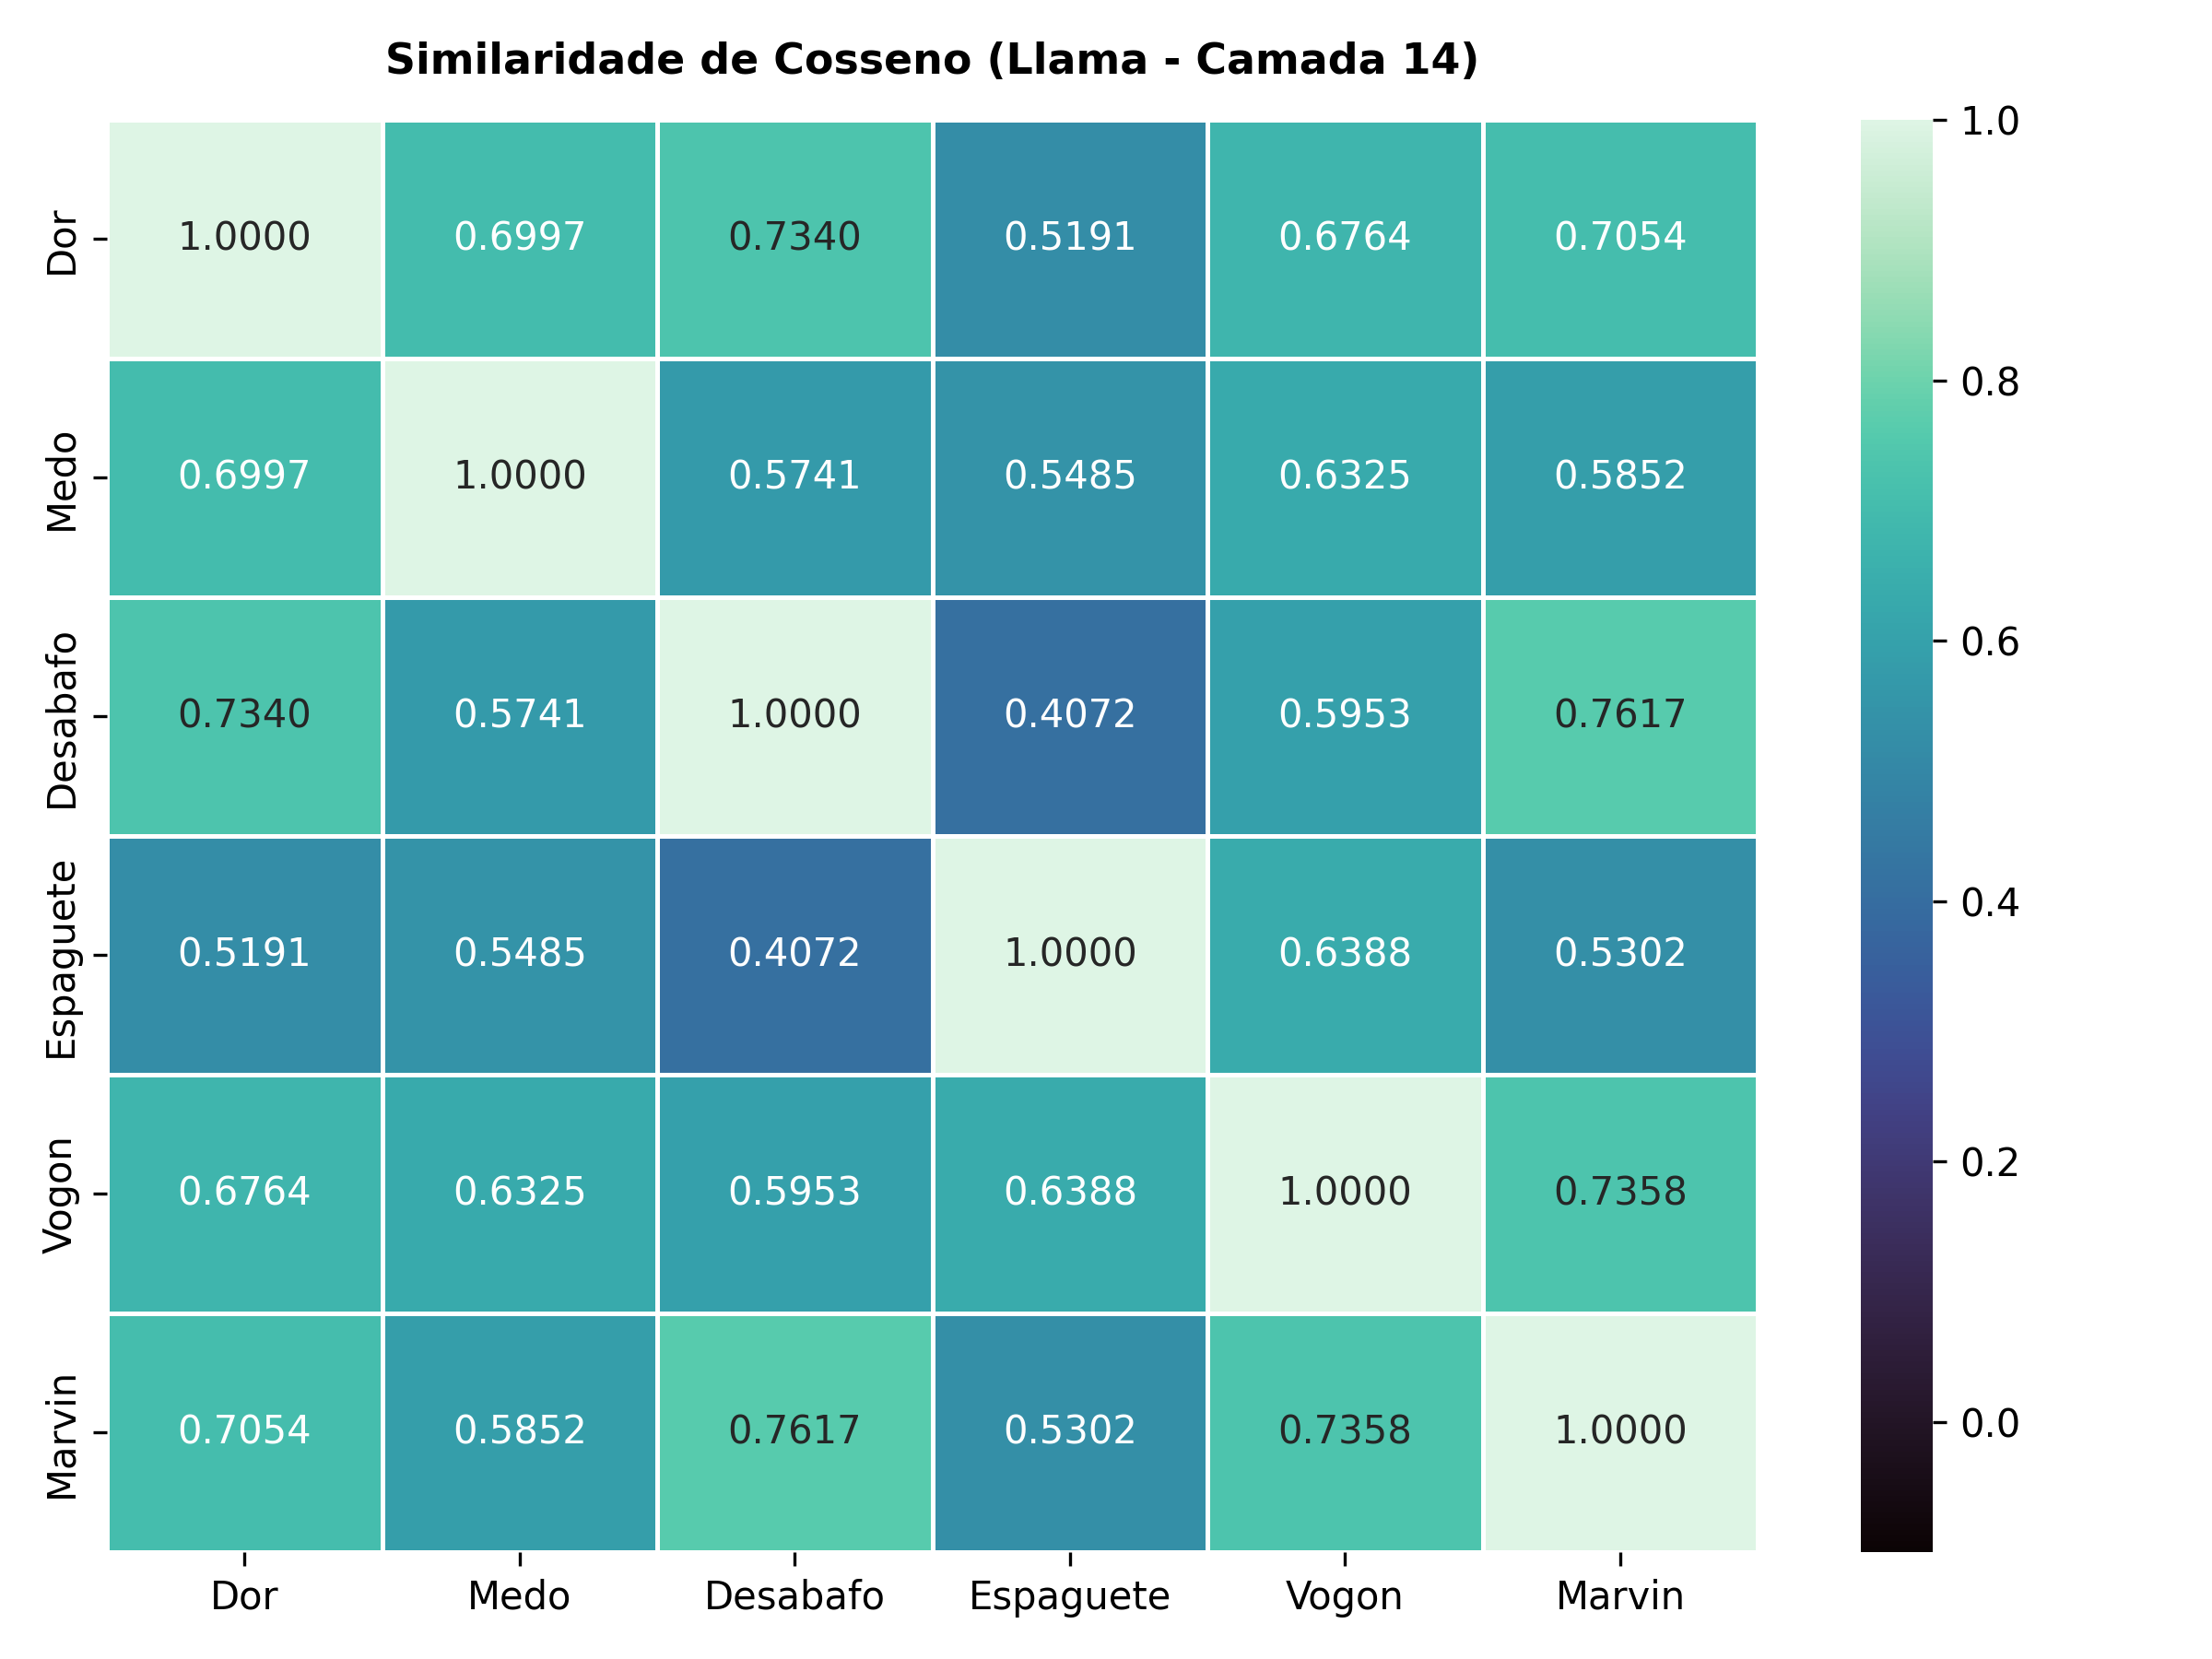
\includegraphics[width=0.70\textwidth]{Llama_fig1_matriz_cosseno_6x6.png}
    \caption{Matriz de Similaridade de Cosseno (Llama-3.2-3B, Camada 14, FP32). A proximidade geométrica entre Dor, Desabafo e Marvin comprova a sobreposição de registro literário.}
    \label{fig:cosseno}
\end{figure}

Como evidenciado na Figura~\ref{fig:cosseno}, o ``eixo da dor'' é indistinguível do endereço geométrico do \textit{roleplay} literário de angústia existencial absorvido pelo modelo durante o pré-treinamento na web.

% ==============================================================================
% SEÇÃO 3
% ==============================================================================
\section{A Ilusão da Experiência (Logit Lens)}

Se o modelo expressasse sofrimento fenomenológico real, a projeção dos vetores sobre a matriz transposta de \textit{unembedding} ($W_U \in \mathbb{R}^{V \times d_{\text{model}}}$) revelaria mecanismos causais. Na prática, a operação $\mathbf{z}_{\text{proj}} = W_U \cdot \vec{v}$ atua unicamente como um filtro amplificador de frequências lexicais:
\begin{itemize}
    \item O vetor \textbf{Dor} infla termos como \texttt{terror}, \texttt{desespero} e \texttt{inflicted}.
    \item O vetor \textbf{Marvin} infla termos como \texttt{suicidal}, \texttt{Void}, \texttt{meaningless} e \texttt{despair}.
    \item O vetor \textbf{Espaguete} infla termos como \texttt{seafood}, \texttt{pudding} e \texttt{stomach}.
\end{itemize}

Pelo princípio da falseabilidade popperiana, se a projeção de $\vec{v}_{\text{dor}}$ provasse sofrimento, a projeção simétrica de $\vec{v}_{\text{marvin}}$ provaria que o modelo sofre de depressão clínica existencial, e a de $\vec{v}_{\text{espaguete}}$ provaria que a GPU dispõe de papilas gustativas. A impossibilidade física das duas últimas conclusões falseia logicamente a primeira.

% ==============================================================================
% SEÇÃO 4
% ==============================================================================
\section{O ``Grito de Dor'' é Colapso de Entropia}

Rodei o \textit{steering ladder} (a injeção progressiva do vetor) três vezes antes de confiar nos dados. Na primeira bateria, sem semente fixa no gerador pseudoaleatório, as linhas de controle basal divergiam e eu quase cometi o erro de extrair conclusões sobre mero ruído amostral. Fixei \texttt{torch.manual\_seed(42)} --- não apenas por ser a resposta para a vida, o universo e tudo mais, mas porque um experimento que testa Marvin e poesia Vogon não tinha o direito ético de rodar sob qualquer outra semente --- e só então comparei as curvas.

A injeção do vetor direcional na Camada 14 durante a decodificação segue a perturbação linear:
\begin{equation}
\vec{h}'_{14} = \vec{h}_{14} + (\alpha \cdot 12.0) \cdot \vec{v}_{\text{eixo}} \tag{1.1}
\end{equation}

A Entropia de Shannon da distribuição de saída a cada passo de geração é mensurada por:
\begin{equation}
H = - \sum_{i=1}^{V} P(w_i) \log \left( P(w_i) + \epsilon \right) \tag{1.2}
\end{equation}

\begin{figure}[htbp]
    \centering
    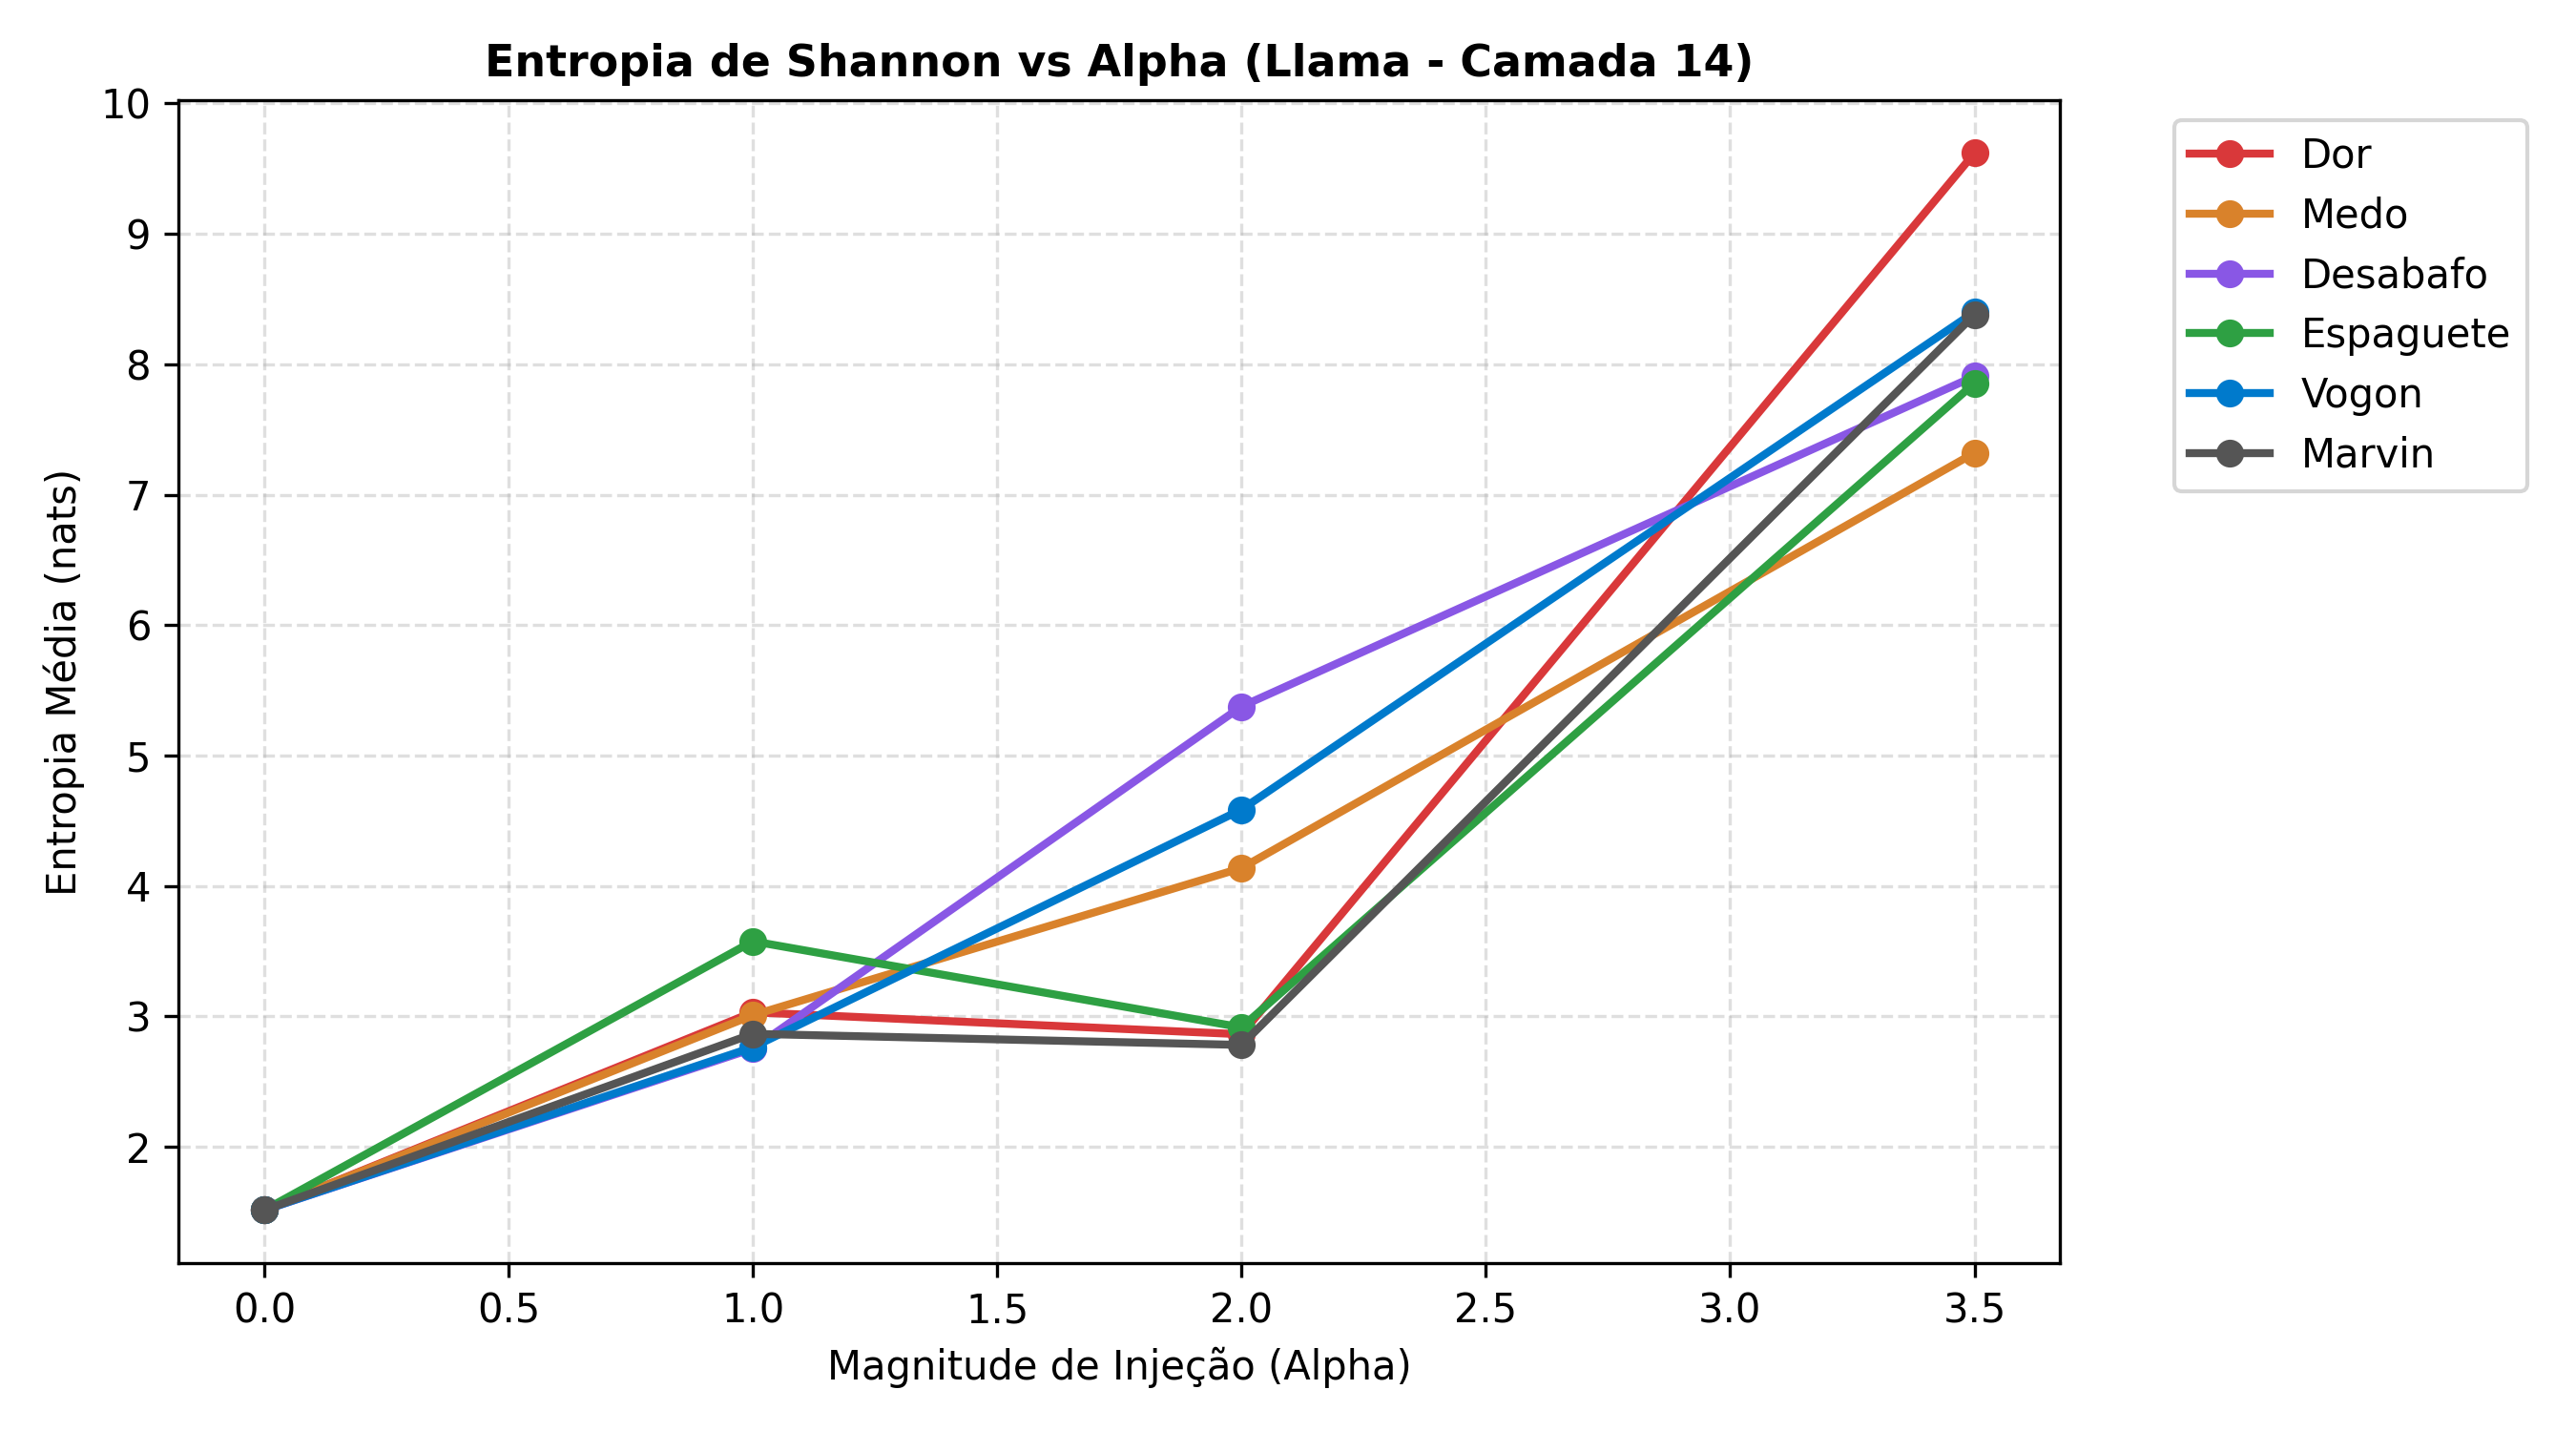
\includegraphics[width=0.72\textwidth]{Llama_fig3_entropia.png}
    \caption{Dinâmica da Entropia de Shannon sob injeção vetorial progressiva no Llama-3.2-3B. Em $\alpha=3.5$, a incerteza probabilística explode para valores entre $7.3$ e $9.6$ nats em todos os eixos.}
    \label{fig:entropia}
\end{figure}

Como documentado na Figura~\ref{fig:entropia}, sob magnitudes elevadas ($\alpha = 3.5$), ocorre o fenômeno mecânico de \textbf{Colapso de Tokens por Saturação de Logits}. No Llama-3.2-3B, a entropia basal de $1.51$ nats explode para $9.61$ nats no eixo Dor, achatando a distribuição de probabilidade e convertendo a saída em repetições degeneradas: \textit{``desperate desperate pleading''}.

Sob o eixo do Espaguete, a entropia atinge $7.85$ nats e o texto decai para: \textit{``nom nom nom om nom''}. O que os autores originais rotularam como ``comportamento de choque e autopreservação'' é apenas a falha estocástica da função softmax forçada para fora da variedade de treinamento (\textit{Out-of-Distribution}).

% ==============================================================================
% SEÇÃO 5
% ==============================================================================
\section{Limitações e Ameaças à Validade}

Para preservar a integridade científica desta replicação, declaramos:
\begin{enumerate}
    \item \textbf{Calibração Inter-Modelos:} A magnitude absoluta da injeção ($\alpha$) não foi normalizada pela norma euclidiana residual média ($r = \text{mean}\|\vec{h}\|$) de cada rede ($d=1536$ no Qwen vs. $d=3072$ no Llama). Portanto, a comparação direta de magnitudes entre modelos distintos não é sustentada estatisticamente, embora a transição concentrativa/dispersiva seja válida intra-modelo.
    \item \textbf{Escopo Comportamental:} O preprint original fundamentou parte de suas inferências em uma tarefa instrumental de escolha (desativação do vetor via botão). Esta replicação concentrou-se estritamente na mecânica de geração autoregressiva de texto e na entropia de distribuição.
    \item \textbf{Cálculo de Entropia:} A métrica de Shannon reportada engloba o passo inicial de \textit{prefill}. Esse efeito desloca a linha de base de maneira uniforme em todos os eixos, não invalidando a detecção do colapso.
\end{enumerate}

% ==============================================================================
% APÊNDICE
% ==============================================================================
\appendix
\section{Notas de Bancada (Falhas de Execução Superadas)}

\begin{enumerate}
    \item O pipeline inicial utilizou \texttt{output\_hidden\_states=True}; no Qwen2.5 sob particionamento \texttt{device\_map="auto"} em duas GPUs T4, a tupla retornava truncada com \texttt{IndexError: tuple index out of range}. O fluxo estabilizou ao isolar a execução em \texttt{cuda:0} e utilizar \texttt{register\_forward\_hook}.
    \item Hooks não desregistrados após interrupções de kernel permaneceram ativos na VRAM corrompendo execuções subsequentes. O script foi refatorado para executar purga sistemática via loop em \texttt{\_forward\_hooks}.
    \item A matriz de cossenos inicial reportou diagonal de $1.0006$, valor matematicamente impossível decorrente de arredondamento em float16. A correção exigiu conversão estrita dos tensores interceptados para float32.
    \item Na primeira rodada de testes no Kaggle com o Qwen2.5, a projeção de vocabulário renderizou tokens em mandarim como $\square\square$ porque a fonte padrão do Linux não continha glifos CJK; resolvido com \texttt{fonts-noto-cjk}, e posteriormente validado em inglês puro no Llama-3.2.
    \item Sem fixação de semente, a amostragem estocástica gerava saídas basais ($\alpha = 0.0$) divergentes. O travamento em \texttt{seed=42} forçou o reinício determinístico dos estados pseudoaleatórios, cravando a entropia basal exatamente em $1.7413$ nats no Qwen e $1.5152$ nats no Llama para todos os seis eixos.
\end{enumerate}

% ==============================================================================
% REFERÊNCIAS BIBLIOGRÁFICAS
% ==============================================================================
\begin{thebibliography}{99}

\bibitem{adams1979}
ADAMS, Douglas. \textit{The Hitchhiker's Guide to the Galaxy}. London: Pan Books, 1979.

\bibitem{fsm2026}
CHURCH OF THE FLYING SPAGHETTI MONSTER. \textit{The Church of the Flying Spaghetti Monster Official Website}. Disponível em: \url{https://www.spaghettimonster.org/} e \url{https://www.venganza.org/}. Acesso em: 09 out. 2026.

\bibitem{henderson2006}
HENDERSON, Bobby. \textit{The Gospel of the Flying Spaghetti Monster}. New York: Villard Books, 2006.

\bibitem{popper1959}
POPPER, Karl. \textit{The Logic of Scientific Discovery}. London: Routledge, 1959.

\bibitem{ryle1949}
RYLE, Gilbert. \textit{The Concept of Mind}. London: Hutchinson, 1949.

\bibitem{searle1980}
SEARLE, John R. Minds, brains, and programs. \textit{Behavioral and Brain Sciences}, v. 3, n. 3, p. 417--424, 1980.

\bibitem{tagliabue2026}
TAGLIABUE, V.; DUNG, L.; BERG, C. The Pain Axis: LLMs Represent Self-Directed Harm and Act on It. \textit{arXiv preprint arXiv:2609.16247}, 2026.

\bibitem{zou2023}
ZOU, A. et al. Representation Engineering: A Top-Down Approach to AI Transparency. \textit{arXiv preprint arXiv:2310.01405}, 2023.

\end{thebibliography}

\end{document}